\section{Estatísticas Gerais}

Nesta seção, são apresentadas as estatísticas gerais dos dados coletados para os dispositivos \textit{Smart-TV} e \textit{Chromecast}. As análises incluem cálculos de medidas descritivas, como média, variância e desvio padrão, além de representações gráficas através de histogramas, boxplots e funções de distribuição empírica (ECDF). 

\subsection{Medidas Descritivas}

As medidas descritivas para as taxas de \textit{upload} e \textit{download} (em escala logarítmica base 10) estão resumidas na Tabela~\ref{tab:estatisticas}. 

\begin{table}[H]
\centering
\caption{Medidas descritivas das taxas de \textit{upload} e \textit{download}.}
\label{tab:estatisticas}
\begin{tabular}{|c|c|c|c|c|}
\hline
\textbf{Dispositivo} & \textbf{Tipo de Tráfego} & \textbf{Média} & \textbf{Variância} & \textbf{Desvio Padrão} \\ \hline
\textit{Smart-TV} & \textit{Upload} & 2.16 & 4.11 & 2.03 \\ \hline
\textit{Smart-TV} & \textit{Download} & 2.35 & 6.72 & 2.59 \\ \hline
\textit{Chromecast} & \textit{Upload} & 3.35 & 0.46 & 0.68 \\ \hline
\textit{Chromecast} & \textit{Download} & 3.80 & 1.66 & 1.29 \\ \hline
\end{tabular}
\end{table}

\subsection{Visualizações Gráficas}

Para compreender melhor a distribuição dos dados, são utilizadas as seguintes representações gráficas:

\begin{itemize}
    \item \textbf{Histogramas:} As distribuições das taxas de \textit{upload} e \textit{download} para cada dispositivo estão representadas nos histogramas da Figura~\ref{fig:histogramas}.
    \item \textbf{Boxplots:} A Figura~\ref{fig:boxplots} mostra os boxplots comparando as taxas de \textit{upload} e \textit{download} entre \textit{Smart-TV} e \textit{Chromecast}.
    \item \textbf{ECDF:} As funções de distribuição empírica, exibidas na Figura~\ref{fig:ecdf}, demonstram a probabilidade acumulada para cada valor das taxas.
\end{itemize}

Para a construção dos histogramas, o número de bins foi calculado utilizando o método de Sturges:

\begin{equation}\label{eq:sturges}
k = 1 + \log_2(n),
\end{equation}

onde \(n\) é o número total de amostras. Este método busca otimizar a visualização dos dados ao balancear granularidade e clareza.

O número de bins calculado para cada dispositivo é o seguinte:
\begin{itemize}
    \item \textbf{\textit{Smart-TV}:} \(k = 24\) bins.
    \item \textbf{\textit{Chromecast}:} \(k = 22\) bins.
\end{itemize}

\begin{figure}[H]
    \centering
    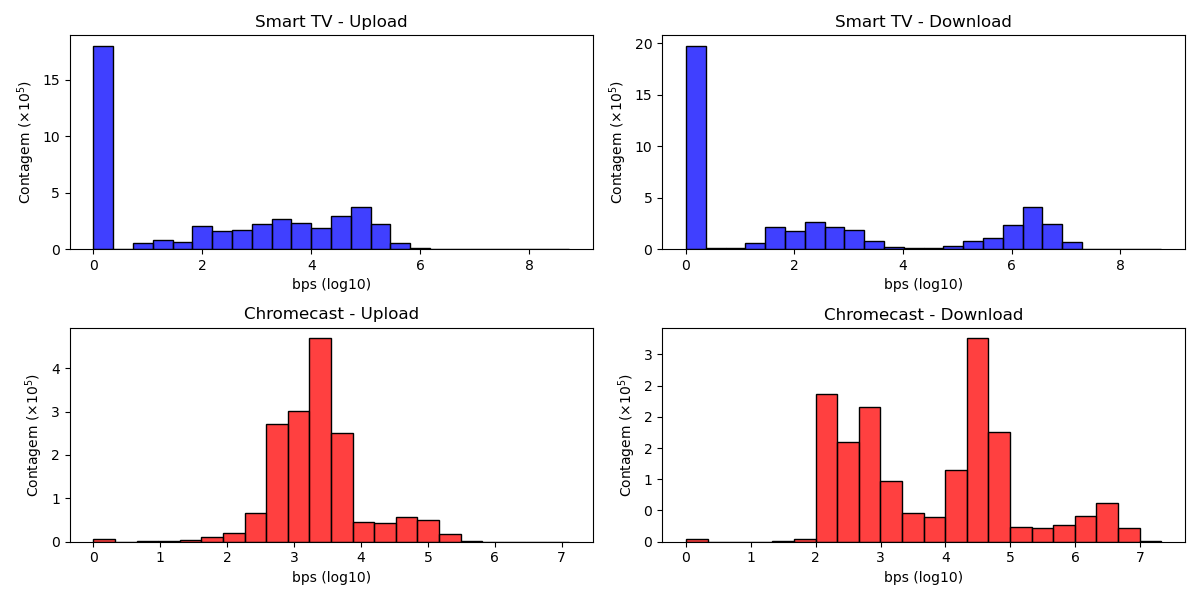
\includegraphics[width=0.8\textwidth]{../estatísticas gerais/histogramas.png}
    \caption{Histogramas das taxas de \textit{upload} e \textit{download} para \textit{Smart-TV} e \textit{Chromecast}.}
    \label{fig:histogramas}
\end{figure}

\begin{figure}[H]
    \centering
    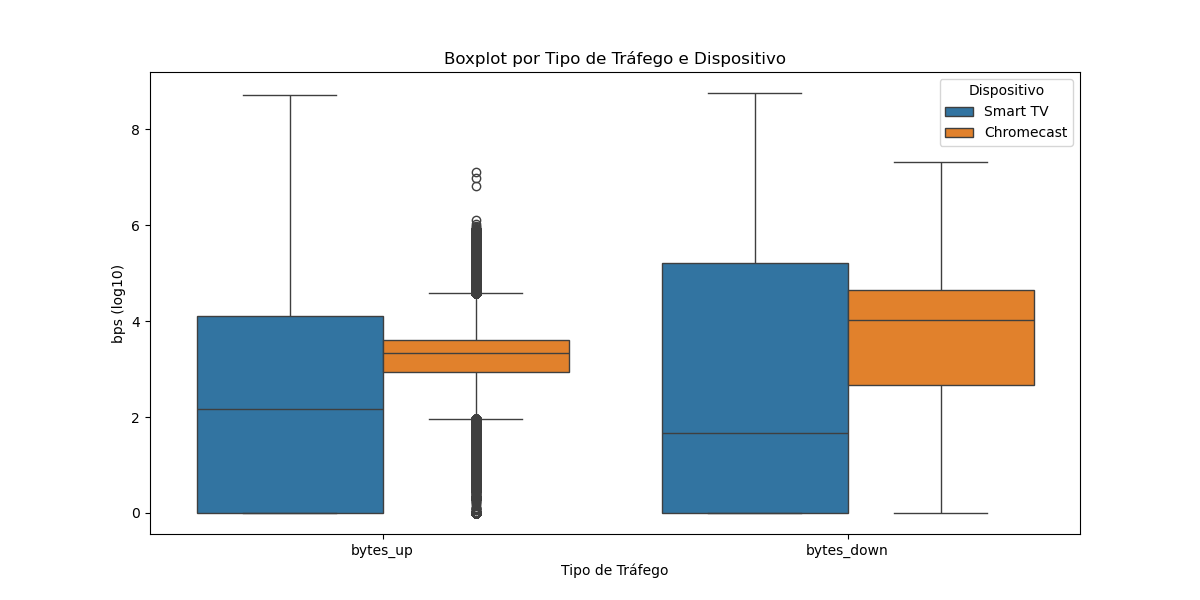
\includegraphics[width=0.8\textwidth]{../estatísticas gerais/boxplot.png}
    \caption{Boxplots das taxas de \textit{upload} e \textit{download} para \textit{Smart-TV} e \textit{Chromecast}.}
    \label{fig:boxplots}
\end{figure}

\begin{figure}[H]
    \centering
    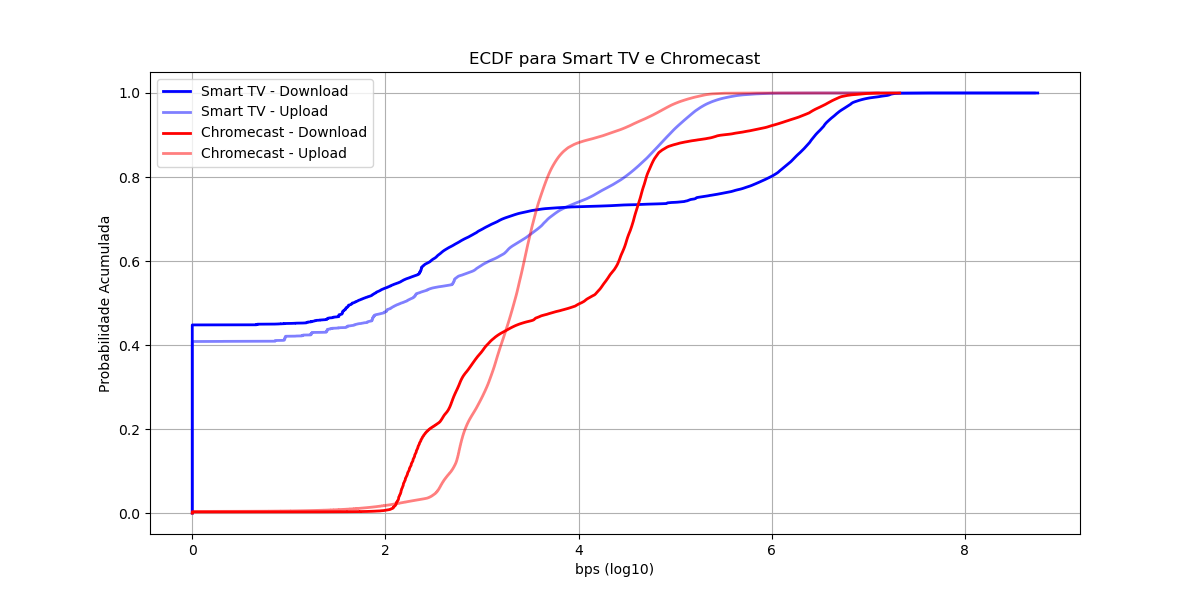
\includegraphics[width=0.8\textwidth]{../estatísticas gerais/ecdf.png}
    \caption{Funções de Distribuição Empírica (ECDF) das taxas de \textit{upload} e \textit{download}.}
    \label{fig:ecdf}
\end{figure}

As visualizações gráficas fornecem informações importantes para o provedor de serviços ao identificar padrões de tráfego específicos de cada dispositivo. Por exemplo, histogramas permitem entender a distribuição predominante de dados, enquanto os boxplots destacam possíveis valores atípicos que podem impactar negativamente a rede. Essas análises auxiliam na definição de prioridades no gerenciamento do tráfego de rede, garantindo uma melhor alocação de recursos para dispositivos com padrões mais variáveis.

\subsection{Análise dos Resultados}

Os resultados destacam diferenças importantes nas características das taxas de \textit{upload} e \textit{download} entre os dispositivos \textit{Smart-TV} e \textit{Chromecast}, com implicações práticas significativas para o provedor de serviços de Internet.

\textbf{\textit{Smart-TV}:} As taxas de \textit{upload} e \textit{download} da \textit{Smart-TV} apresentam médias similares e variâncias relativamente altas, refletindo maior dispersão dos dados. A alta concentração de valores baixos, especialmente iguais a zero, é evidenciada pela primeira barra dominante nos histogramas (Figura~\ref{fig:histogramas}) e pela ECDF inicial, que ultrapassa 0.4 devido aos valores nulos. O boxplot (Figura~\ref{fig:boxplots}) confirma a ausência de outliers, indicando que o tráfego da \textit{Smart-TV} é caracterizado por períodos de inatividade alternados com picos de alta demanda. 

\textbf{\textit{Chromecast}:} O \textit{Chromecast} apresenta padrões diferentes, com taxas de \textit{upload} e \textit{download} mais consistentes e desvios padrão menores. Embora a taxa de \textit{download} não tenha outliers, a taxa de \textit{upload} exibe diversos picos e vales, refletidos nos boxplots. A ECDF mostra um crescimento rápido após \(10^2\) bps, indicando concentração em valores intermediários e reforçando o comportamento mais estável do dispositivo.

\textbf{Comparação Geral:} Enquanto a \textit{Smart-TV} alterna entre inatividade e fluxos intensos, o \textit{Chromecast} mantém tráfego mais constante, mas com picos significativos no \textit{upload}. Essas diferenças sugerem abordagens específicas para otimização da rede: adaptar a alocação de recursos às demandas variáveis da \textit{Smart-TV} e conter os picos do \textit{Chromecast}, priorizando a estabilidade.

\textbf{Implicações Práticas:} Os padrões observados podem ajudar o provedor de serviços a otimizar sua infraestrutura. Para a \textit{Smart-TV}, estratégias adaptativas para lidar com períodos de alta demanda podem reduzir a sobrecarga durante picos. Já para o \textit{Chromecast}, sistemas de contenção que lidem com os picos de \textit{upload} podem evitar saturação da rede. A implementação dessas políticas pode melhorar a eficiência operacional e a qualidade da experiência (QoE) do usuário final.
